% The two cleanup stages: restoration on top, smoothing below.
% Render: pdflatex -interaction=nonstopmode diagram_cleanup_stages.tex
% Then:  pdftoppm -png -r 400 -singlefile diagram_cleanup_stages.pdf out
% The picture is exactly \textwidth wide, so the deck places it with width=\linewidth.
\documentclass[border=0pt,11pt]{standalone}
\usepackage[T1]{fontenc}
\usepackage[utf8]{inputenc}
\usepackage{helvet}
\renewcommand{\familydefault}{\sfdefault}
\usepackage{tikz}
\usetikzlibrary{positioning,arrows.meta}

\definecolor{primaryNavy}{RGB}{24,24,27}
\definecolor{secondaryNavy}{RGB}{63,63,70}
\definecolor{mutedGray}{RGB}{248,250,252}
\definecolor{ruleGray}{RGB}{226,232,240}

\tikzset{
  proc/.style={draw=secondaryNavy,line width=0.5pt,fill=mutedGray,text=primaryNavy,
               font=\small,align=center,inner xsep=4pt,inner ysep=3.5pt,
               minimum height=0.62cm,minimum width=1cm},
  rowlbl/.style={text=secondaryNavy,font=\footnotesize,align=right,inner sep=1pt},
  fl/.style={draw=secondaryNavy,line width=0.6pt,
             -{Stealth[length=1.7mm,width=1.4mm]}},
}

\begin{document}
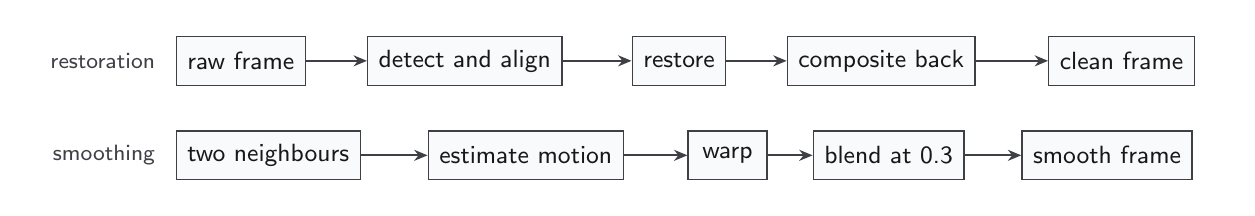
\begin{tikzpicture}
\useasboundingbox (-0.0285cm,-1.6140cm) rectangle (-0.0285cm+433.34402pt,0.4212cm);
\fill[white] (-0.0285cm,-1.6140cm) rectangle (-0.0285cm+433.34402pt,0.4212cm);

% ---- row labels ------------------------------------------------------------
\node[rowlbl,anchor=east] at (1.63,0) {restoration};
\node[rowlbl,anchor=east] at (1.63,-1.2) {smoothing};

% ---- row 1: restore --------------------------------------------------------
\node[proc,anchor=west] (r1a) at (1.85,0)    {raw frame};
\node[proc,anchor=west] (r1b) at (4.28,0)    {detect and align};
\node[proc,anchor=west] (r1c) at (7.64,0)    {restore};
\node[proc,anchor=west] (r1d) at (9.61,0)    {composite back};
\node[proc,anchor=west] (r1e) at (12.93,0)   {clean frame};
\draw[fl] (r1a) -- (r1b);
\draw[fl] (r1b) -- (r1c);
\draw[fl] (r1c) -- (r1d);
\draw[fl] (r1d) -- (r1e);

% ---- row 2: smooth ---------------------------------------------------------
\node[proc,anchor=west] (r2a) at (1.85,-1.2)  {two neighbours};
\node[proc,anchor=west] (r2b) at (5.05,-1.2)  {estimate motion};
\node[proc,anchor=west] (r2c) at (8.35,-1.2)  {warp};
\node[proc,anchor=west] (r2d) at (9.94,-1.2)  {blend at 0.3};
\node[proc,anchor=west] (r2e) at (12.59,-1.2) {smooth frame};
\draw[fl] (r2a) -- (r2b);
\draw[fl] (r2b) -- (r2c);
\draw[fl] (r2c) -- (r2d);
\draw[fl] (r2d) -- (r2e);
\end{tikzpicture}
\end{document}
